\section{The Biot-Savart Law and a Straight Wire}
\label{biot_savart_straight_wire}

\instructornote{%
By Matt Trawick, 2015.   Time: 30 minutes
}

\makelabheader %(Space for student name, etc., defined in master.tex)

\vspace{0.5cm}

\textbf{Objective and statement of the problem:}

Find the magnetic field $\vv{B}$ at a point $P$ which is a distance $y$ away from the midpoint of a thin wire of length $L$ carrying current $I$.
\begin{center}
    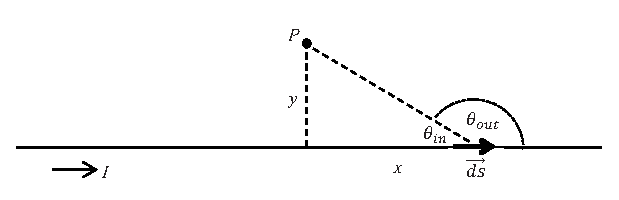
\includegraphics[width=0.7\textwidth]{biot_savart_straight_wire/straight_wire.eps}
\end{center}

\textbf{Introduction and outline of solution:}
We'll divide the wire into a bunch of short lengths $\vv{ds}$, and calculate the field at $P$ using the Biot-Savart law:
\begin{displaymath}
\vv{B} = \int{\frac{\mu_0I}{4 \pi}\frac{\vv{ds}\times \hat{r}}{r^2}}
\end{displaymath}

\textbf{Step 1:} \newline
Let's make the $x$-axis along the wire, with $x=0$ just below $P$.  What is the distance $r$ in the Biot-Savart law, in terms of $x$ and $y$ on the drawing?

\vspace{.6in}


\textbf{Step 2:} \newline
What is the direction of the vectors $\vv{r}$ and $\hat{r}$?



\vspace{.6in}

\textbf{Step 3:} \newline
What is the direction of  $\vv{ds}\times \hat{r}$?  Is the direction the same for all $\vv{ds}$ along the wire? 

\vspace{.6in}


\textbf{Step 4:} \newline
You know that $\left|\vv{ds}\times \hat{r}\right|=\left|\vv{ds}\right|  \left|\hat{r}\right|\sin\theta$.  Which $\theta$ is the one you want, $\theta_{in}$ or $\theta_{out}$?

\vspace{.6in}

\textbf{Step 5:} \newline
In fact, which is bigger: $\sin \theta_{in}$ or $\sin \theta_{out}$, or are they the same?

\newpage

\textbf{Step 6:} \newline
Combine your answers from steps 1 through 5 to rewrite the Biot-Savart law so that the cross product is gone and all geometric variables are in terms of $x$ and $y$. (What variable are you integrating over, anyway?) 

\vspace{1.0in}

\textbf{Step 7:} \newline
Evaluate the integral, remembering your limits of integration.  


 \vfill

\textbf{Step 8:} \newline
Just out of curiosity, what does your answer reduce to in the limit $L\longrightarrow\infty$?

\vspace{1.0in}


\textit{Note: one of the following might be helpful:}
\begin{flalign*}
& \int \! \frac{1}{\left (u^2 + a^2 \right )^\frac{3}{2}} \, du=\frac{u}{a^2 \sqrt{u^2 + a^2}} &\\
& \int \! \frac{u}{\left (u^2 + a^2 \right )^\frac{3}{2}} \, du=\frac{-1}{\sqrt{u^2 + a^2}} \\
& \int \! \frac{1}{u^2 + a^2} \, du=\frac{1}{a} \tan^{-1} \frac{u}{a}
\end{flalign*}


